%\setchapterimage{bandeau}
\chapter*{Application \arabic{cptApplication} \\ 
Réglage de correcteurs P et AP -- 
\ifprof Corrigé \else Sujet \fi}
\addcontentsline{toc}{section}{Application \arabic{cptApplication} :
Réglage de correcteurs P et AP -- 
\ifprof Corrigé \else Sujet \fi}

\iflivret \stepcounter{cptApplication} \else
\ifprof  \stepcounter{cptApplication} \else \fi
\fi

\setcounter{question}{0}
\marginnote{Ressources de P. Dupas.}
\marginnote[1cm]{
\UPSTIcompetence[2]{C1-02}
\UPSTIcompetence[2]{C2-04}}





\subsection*{Correcteur proportionnel}
Soit un système de fonction de transfert $G(p)=\dfrac{1}{\left(1+10p\right)\left(1+0,1p\right)\left(1+0,2p\right)}$ placé dans une boucle à retour unitaire.

\question{Déterminer la précision du système $\varepsilon_S$ pour une entrée échelon unitaire.}
\ifprof
\begin{corrige}
Le système est de classe 0. L'entrée est de type échelon. $K_{\text{BO}}=1$.
L'écart statique est de $\dfrac{1}{1+1}=\dfrac{1}{2}$.
\end{corrige}
\else
\fi

\question{Justifier le tracer du diagramme de Bode de la fonction de transfert en boucle ouverte du système.}
\ifprof
\begin{corrige}
\begin{center}
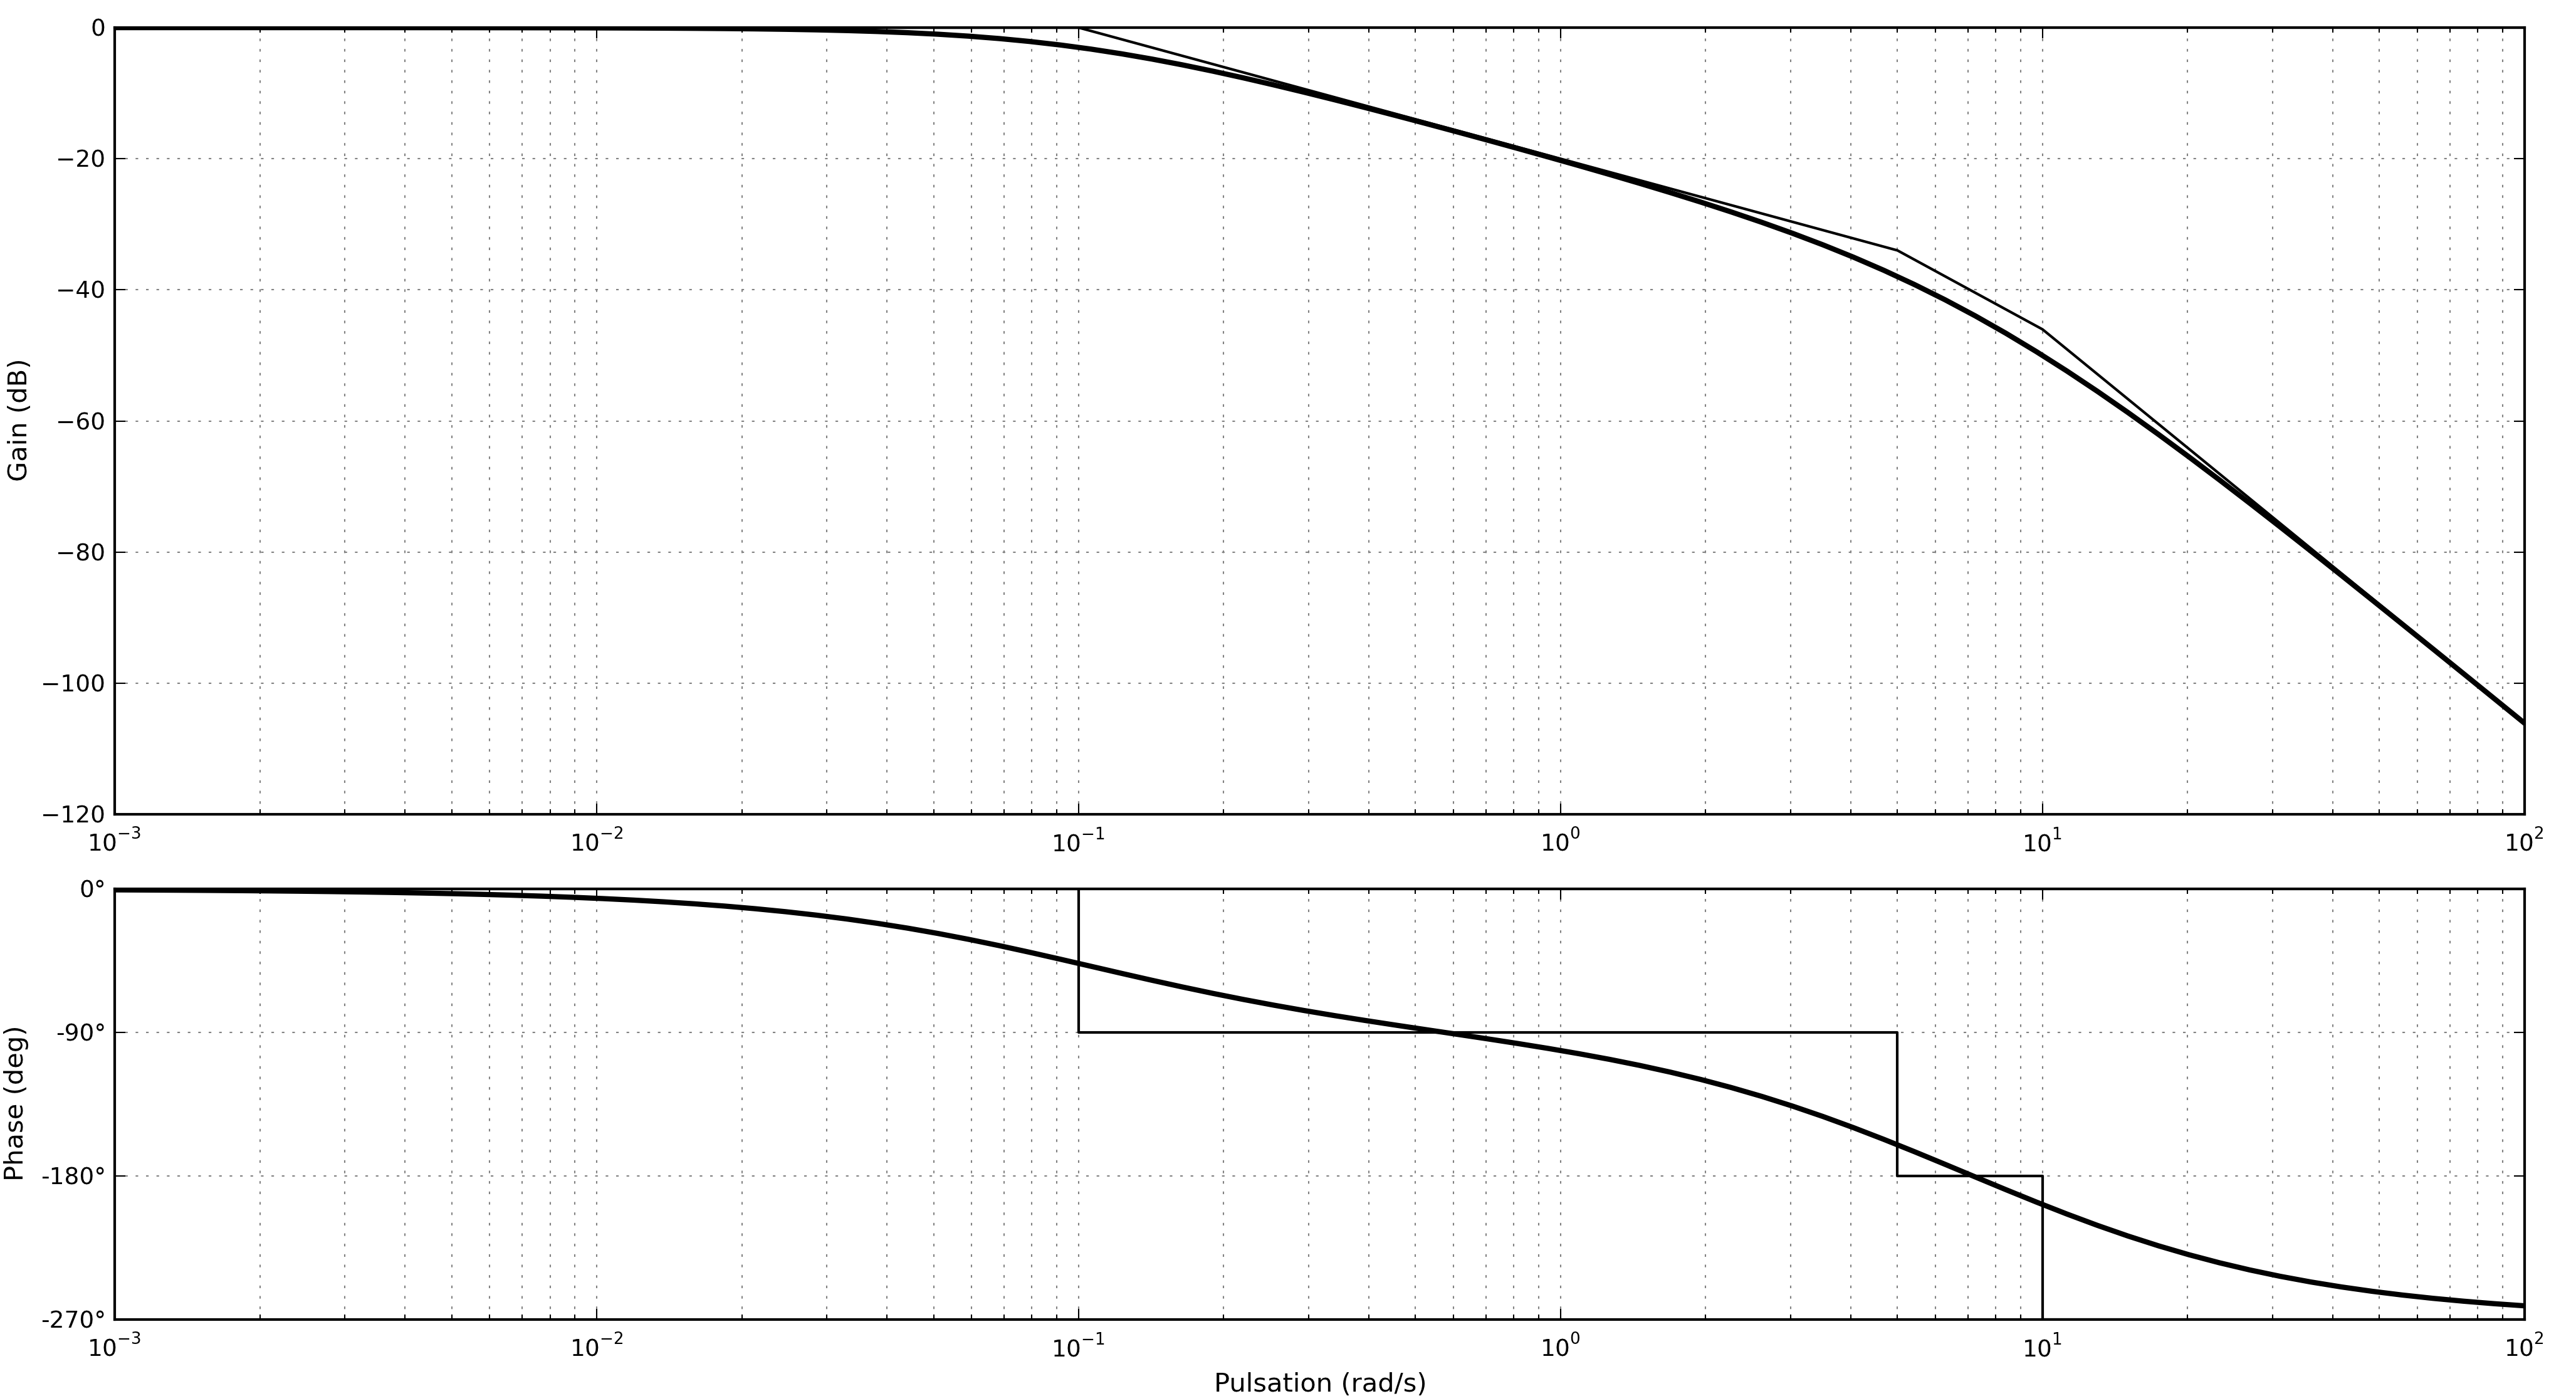
\includegraphics[width=.9\linewidth]{01_Bode}
\end{center}
\end{corrige}
\else
\begin{center}
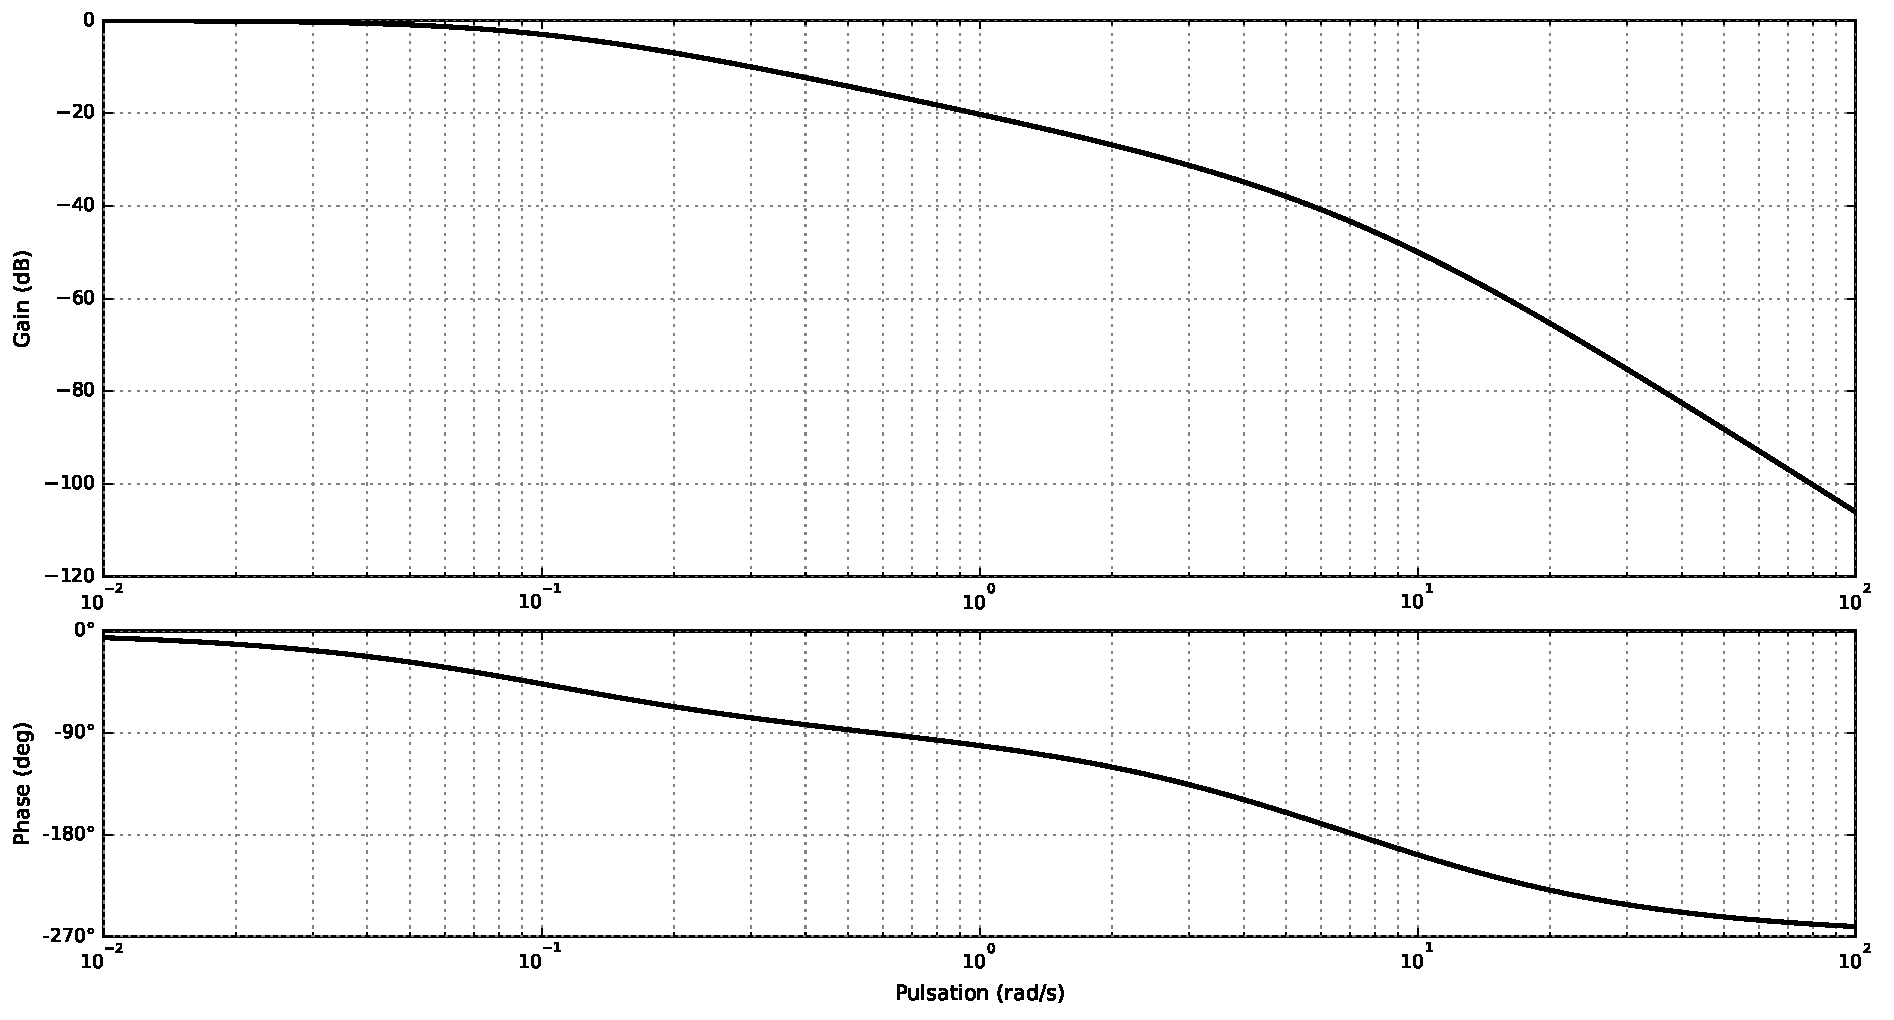
\includegraphics[width=\linewidth]{01_exo_01_bode}
\end{center}
\fi


\question{Déterminer $K$ pour avoir une marge de phase de 45\degres. Indiquer alors la valeur de la marge de gain. Indiquer la valeur de l'écart statique.}

\ifprof
\begin{corrige} ~\\

\begin{itemize}
\item On résout $\varphi\left(\omega\right)=-135\degres$ : 
$\varphi\left(\omega\right)=-\arctan 10\omega-\arctan 0,1\omega-\arctan 0,2\omega$.

$\varphi\left(\omega\right)=-135\degres \Leftrightarrow \omega = \SI{2,95}{rad.s^{-1}}$ (solveur Excel). 

\item Calculons $G_{\text{dB}}(\omega)=-20\log\left(\sqrt{1+10^2\omega^2} \right)-20\log\left(\sqrt{1+0,1^2\omega^2} \right)-20\log\left(\sqrt{1+0,2^2\omega^2} \right)=\SI{-31}{dB}$. Il faut donc augmenter le gain de \SI{31}{dB} soit $K_P=10^{31/20}=35,48$.


\item On a alors un écart statique de $\dfrac{1}{1+35,48}=0,027$.

\item Pour déterminer la marge de gain, il faut résoudre $\varphi\left(\omega\right)=-180\degres$. On obtient $\omega=\SI{7,17}{rad/s}$ et $M_G=\SI{12}{dB}$.
\end{itemize}


\begin{center}
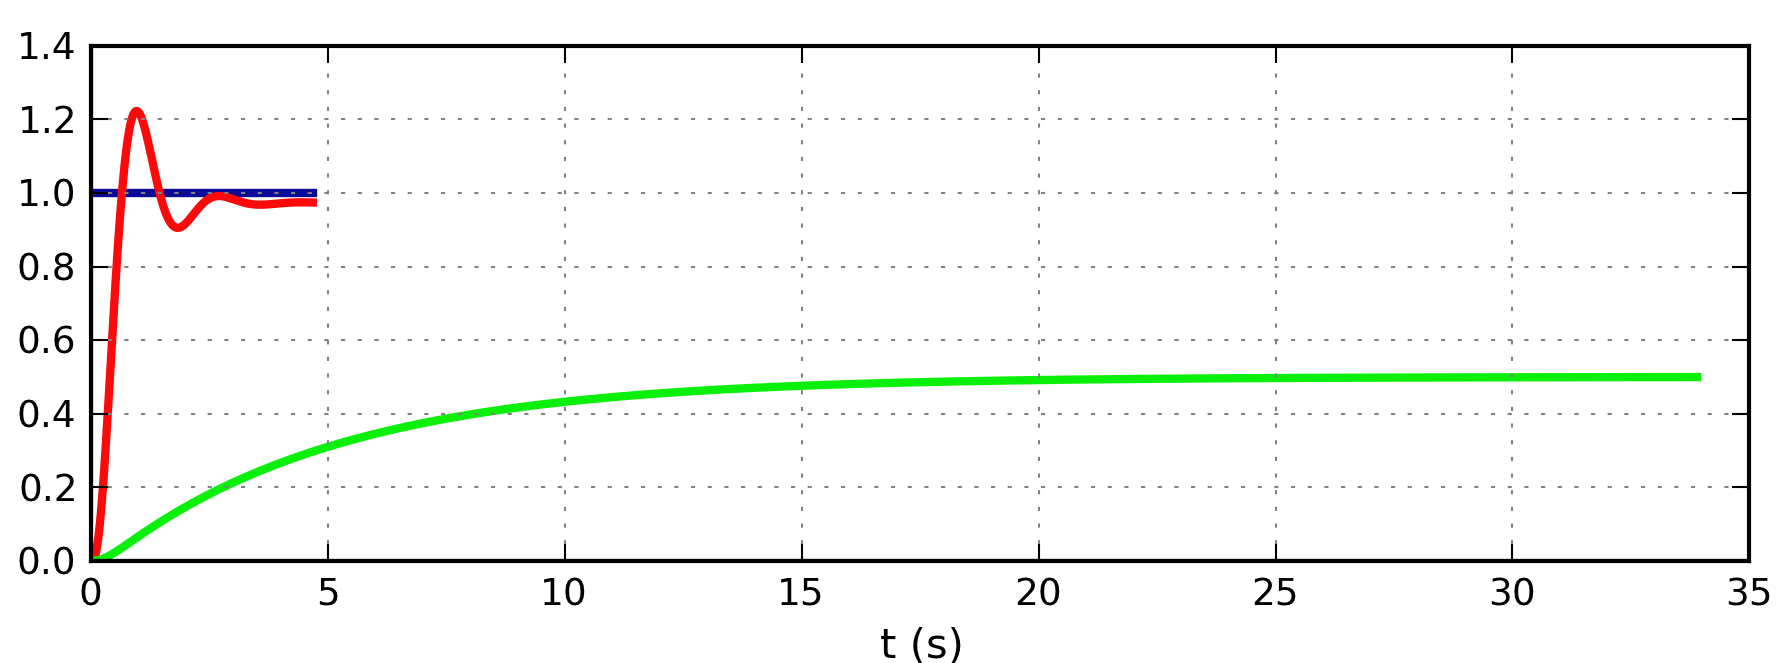
\includegraphics[width=.9\linewidth]{01_02}
\end{center}

\end{corrige}
\else
\fi


\question{Déterminer $K$ pour avoir une marge de gain de \SI{6}{dB}. Indiquer alors la valeur de l'écart statique.}
\ifprof
\begin{corrige}
\begin{itemize}
\item On commence par résoudre $\varphi\left(\omega\right)=-180\degres$. On obtient $\omega=\SI{7,17}{rad/s}$ et $M_G=\SI{44}{dB}$.

\item Il faut augmenter le gain de \SI{38}{dB} soit $20\log K_P=38\Rightarrow K_P=10^{38/20}=79$.


\item On a alors un écart statique de $\dfrac{1}{1+79}=0,0125$.

\item La marge de phase est alors de 19\degres. 
\end{itemize}

\begin{center}
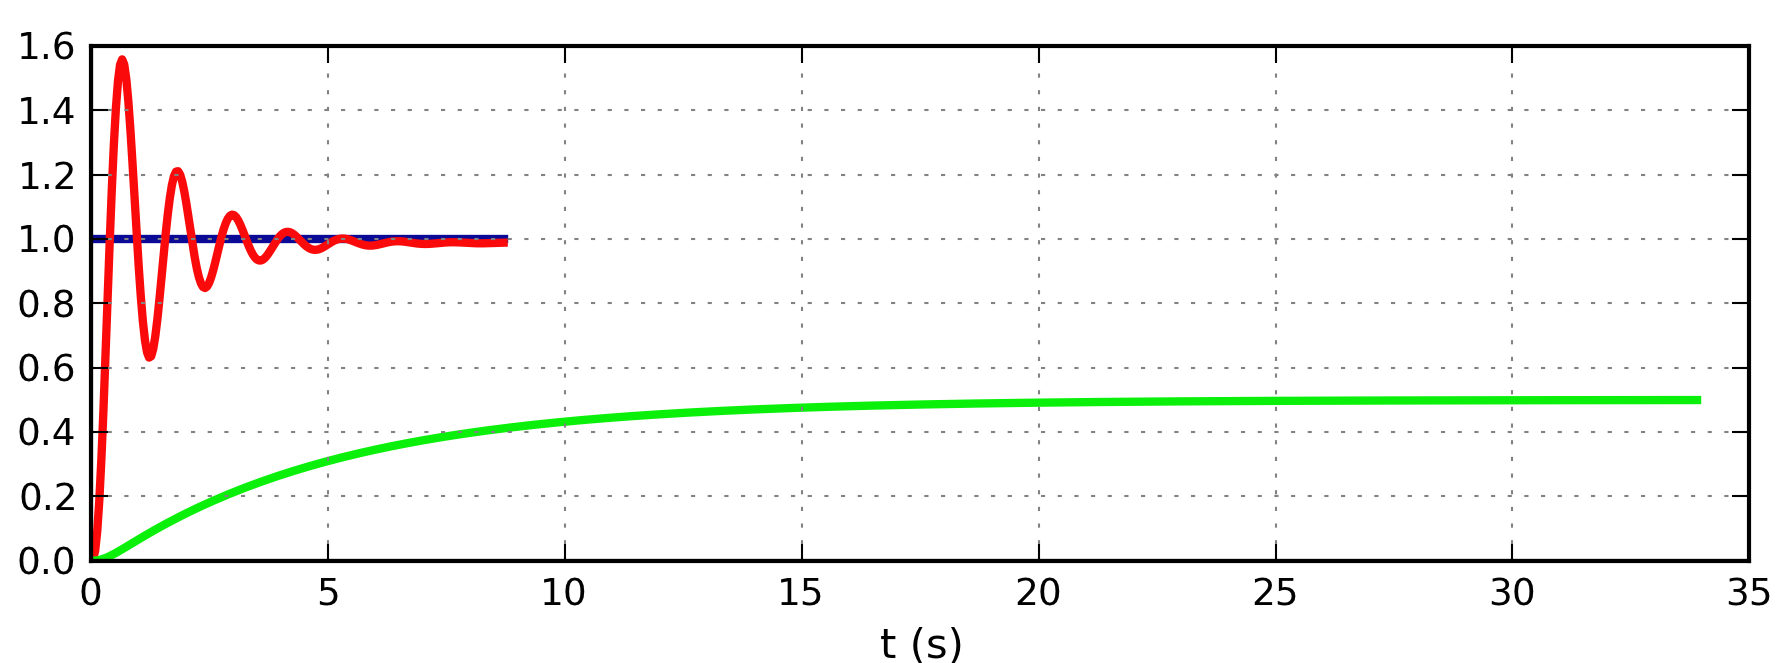
\includegraphics[width=.9\linewidth]{01_03}
\end{center}

\end{corrige}
\else
\fi



\ifprof
\else
\ifcolle
\else
\marginnote{
\begin{solution}
\begin{enumerate}
\item $\varepsilon_S=\dfrac{1}{2}$.
\item $\quad$.
\item $\omega_{-135\degres}=\SI{2,95}{rad/s}$.
\item $\omega_{\SI{0}{dB}}=\SI{7,17}{rad/s}$ et $M_G=\SI{38}{dB}$ soit $K_P=79$.
\end{enumerate} 
\end{solution}}
\fi
\fi

%\end{multicols}


%\ifprof
%\else
%\begin{center}
%\rotatebox{90}{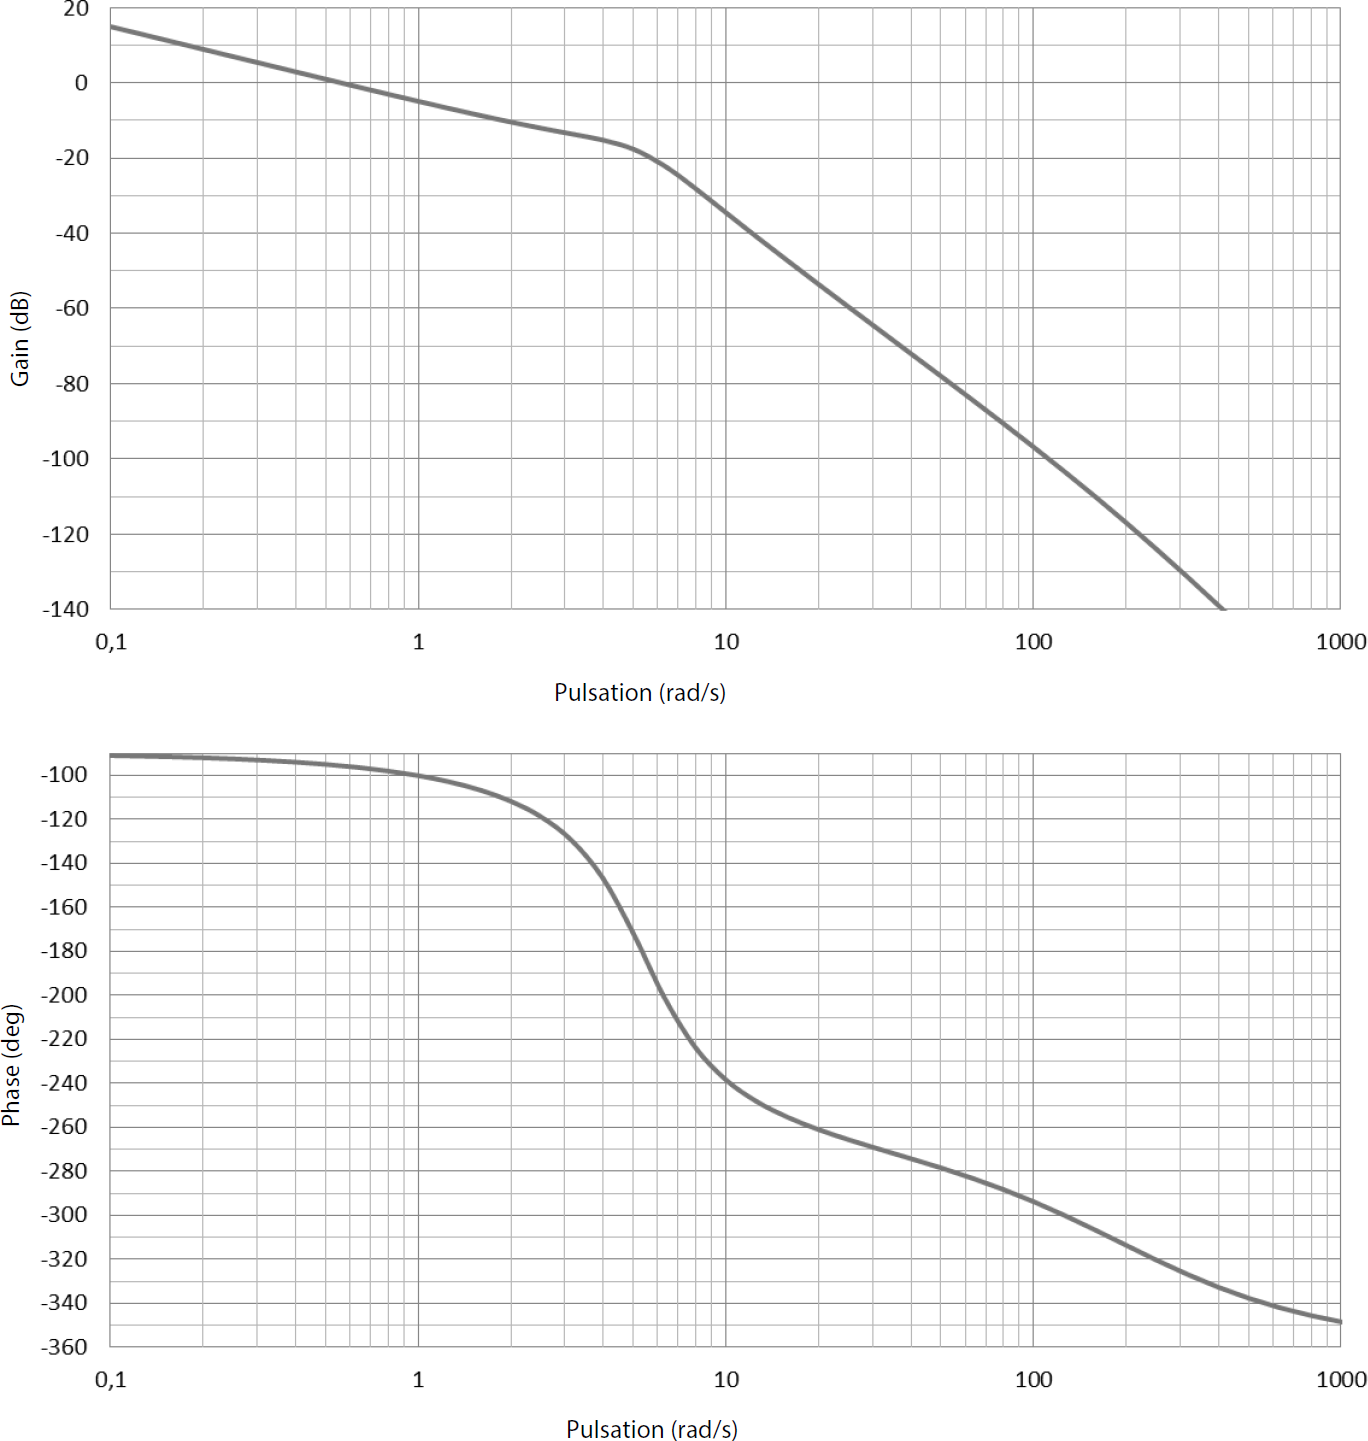
\includegraphics[width=.8\linewidth]{fig_04}}
%\end{center}
%\fi



\subsection*{Correcteur à avance de phase}

Soit un système de fonction de transfert $G(p)=\dfrac{100}{\left(p+1\right)^2}$ placé dans une boucle à retour unitaire. On souhaite corrige ce système en utilisant un correcteur à avance de phase de la forme $C(p)=K\dfrac{1+a\tau p}{1+\tau p}$.


\question{Justifier le tracer du diagramme de Bode de $G(p)$.}

\begin{center}
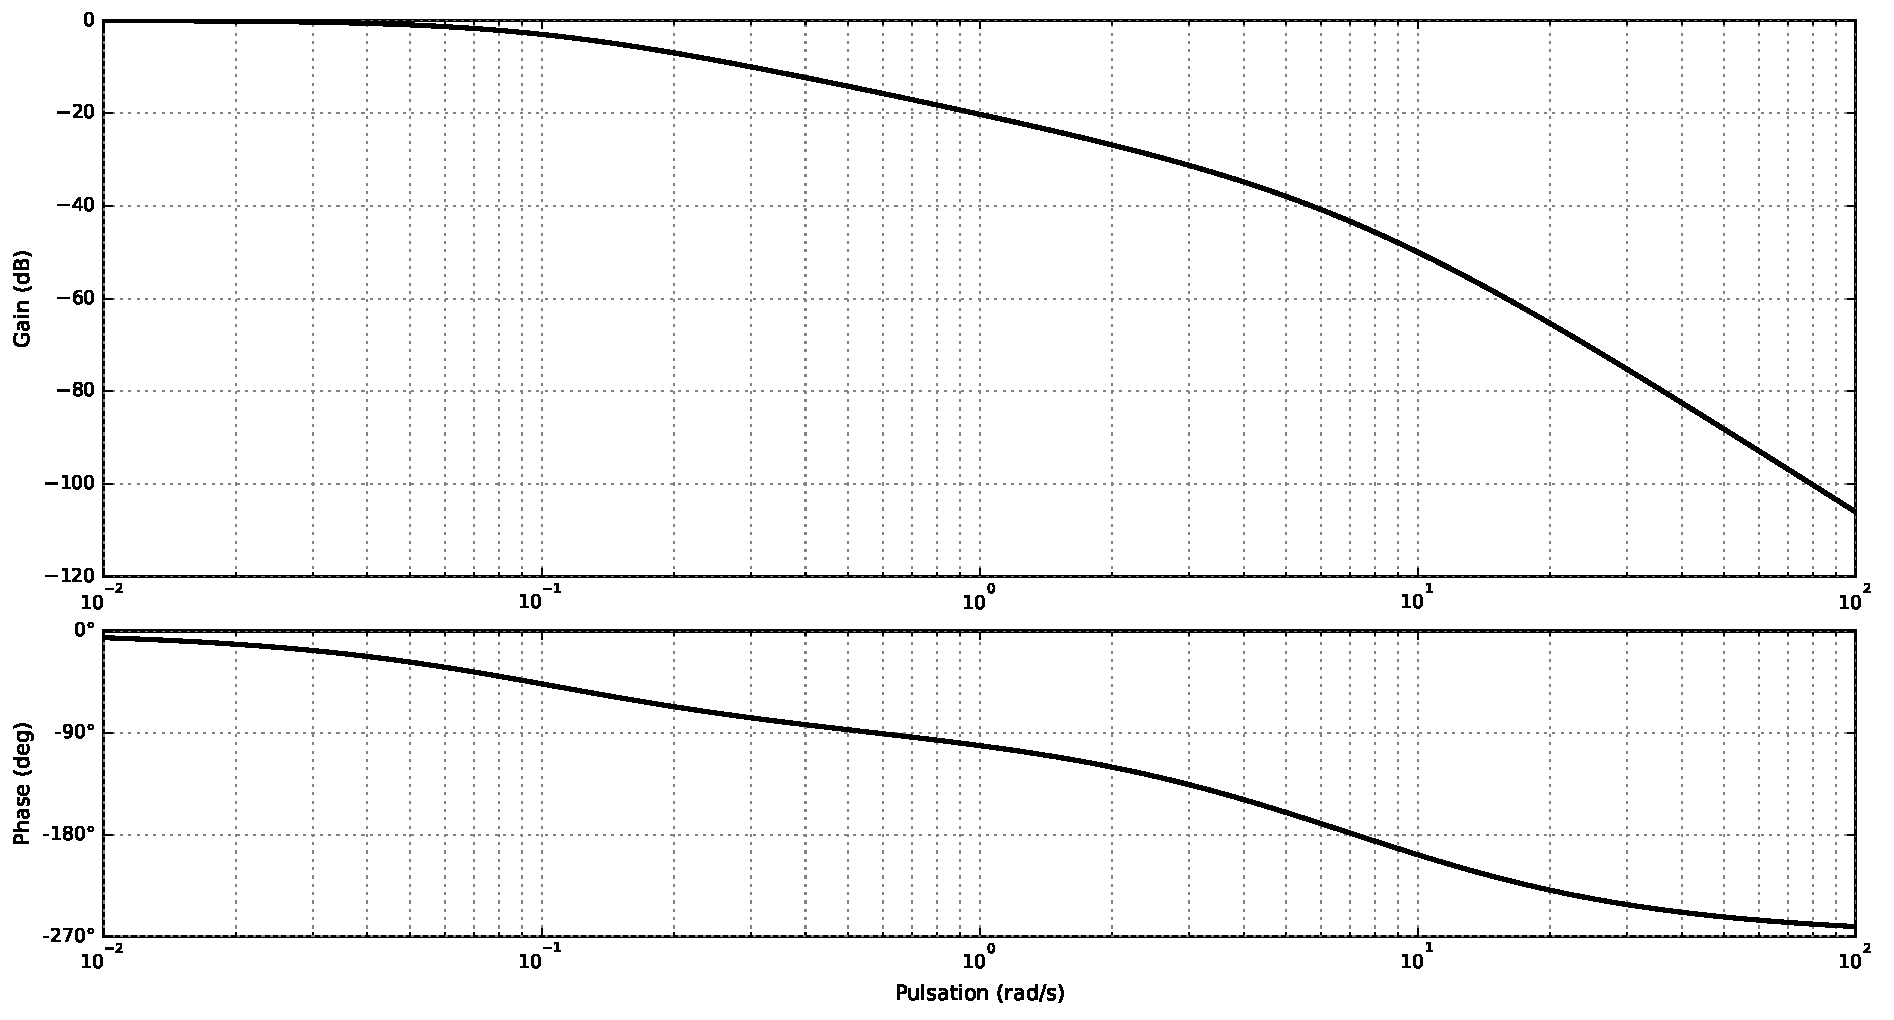
\includegraphics[width=\linewidth]{01_exo_01_bode}
\end{center}

\question{Corriger ce système de sorte que sa marge de phase soit égale à 45\degres.}
\ifprof
\begin{corrige}~\\
\begin{itemize}
\item $G_{\text{dB}}(\omega)=20\log \left(100\right)-20\log\left(1+\omega^2\right)$. $G_{\text{dB}}(\omega)=0 \Leftrightarrow \dfrac{100}{1+\omega^2}=1$ $  \Leftrightarrow \omega=\pm\sqrt{99}$ $\Rightarrow \omega=\SI{9,95}{rad/s}$.
\item $\varphi(\omega)=-2\arctan\omega$ et $\varphi(9,95)=-\SI{2,94}{rad}=-169\degres$ soit une marge de phase de 11\degres; le correcteur doit donc apporter un complément de phase de 34\degres. 
\item $\varphi_{\text{max}}=\arcsin\left( \dfrac{a-1}{a+1}\right)\Rightarrow \sin \left(\varphi_{\text{max}}\right)=\dfrac{a-1}{a+1}$ 
$\Rightarrow a=-\dfrac{\sin \left(\varphi_{\text{max}}\right)+1}{ \sin \left(\varphi_{\text{max}}\right) -1}=3,54$.
\item $\tau=\dfrac{1}{9,95\sqrt{3,54}}=\SI{0,053}{s}$.
\end{itemize}
\end{corrige}
%\ifprof
%\begin{itemize}
%\item Pulsation de coupure à \SI{0}{dB} su système non corrigé en BO : $\omega=\SI{9,95}{rad.s^{-1}}$.
%\item Pour cette pulsation la marge de phase est de 11\degres.
%\item On cherche $\varphi_{\text{max}}=25\degres$ et $a=3,54$. 
%\item $\omega_{\text{max}}=\SI{9,95}{rad.s^{-1}}= \dfrac{1}{T\sqrt{a}}$ %ce qui conduit à $T=\SI{0,053}{s}$.
%\item $K=\dfrac{1}{\sqrt{a}}=0,53$.
%\end{itemize}
\else
\fi


\question{Tracer le diagramme de Bode du correcteur et le diagramme de la boucle ouverte corrigée.}
\ifcolle
\else
\marginnote{
\begin{solution}
\begin{enumerate}
\item $\quad$
\item $C(p)=0,53\dfrac{1+3,54 \cdot 0,053  p}{1+0,053 p}$.
\item $\quad$
\end{enumerate}
\end{solution}}
\fi



\ifprof
\begin{center}
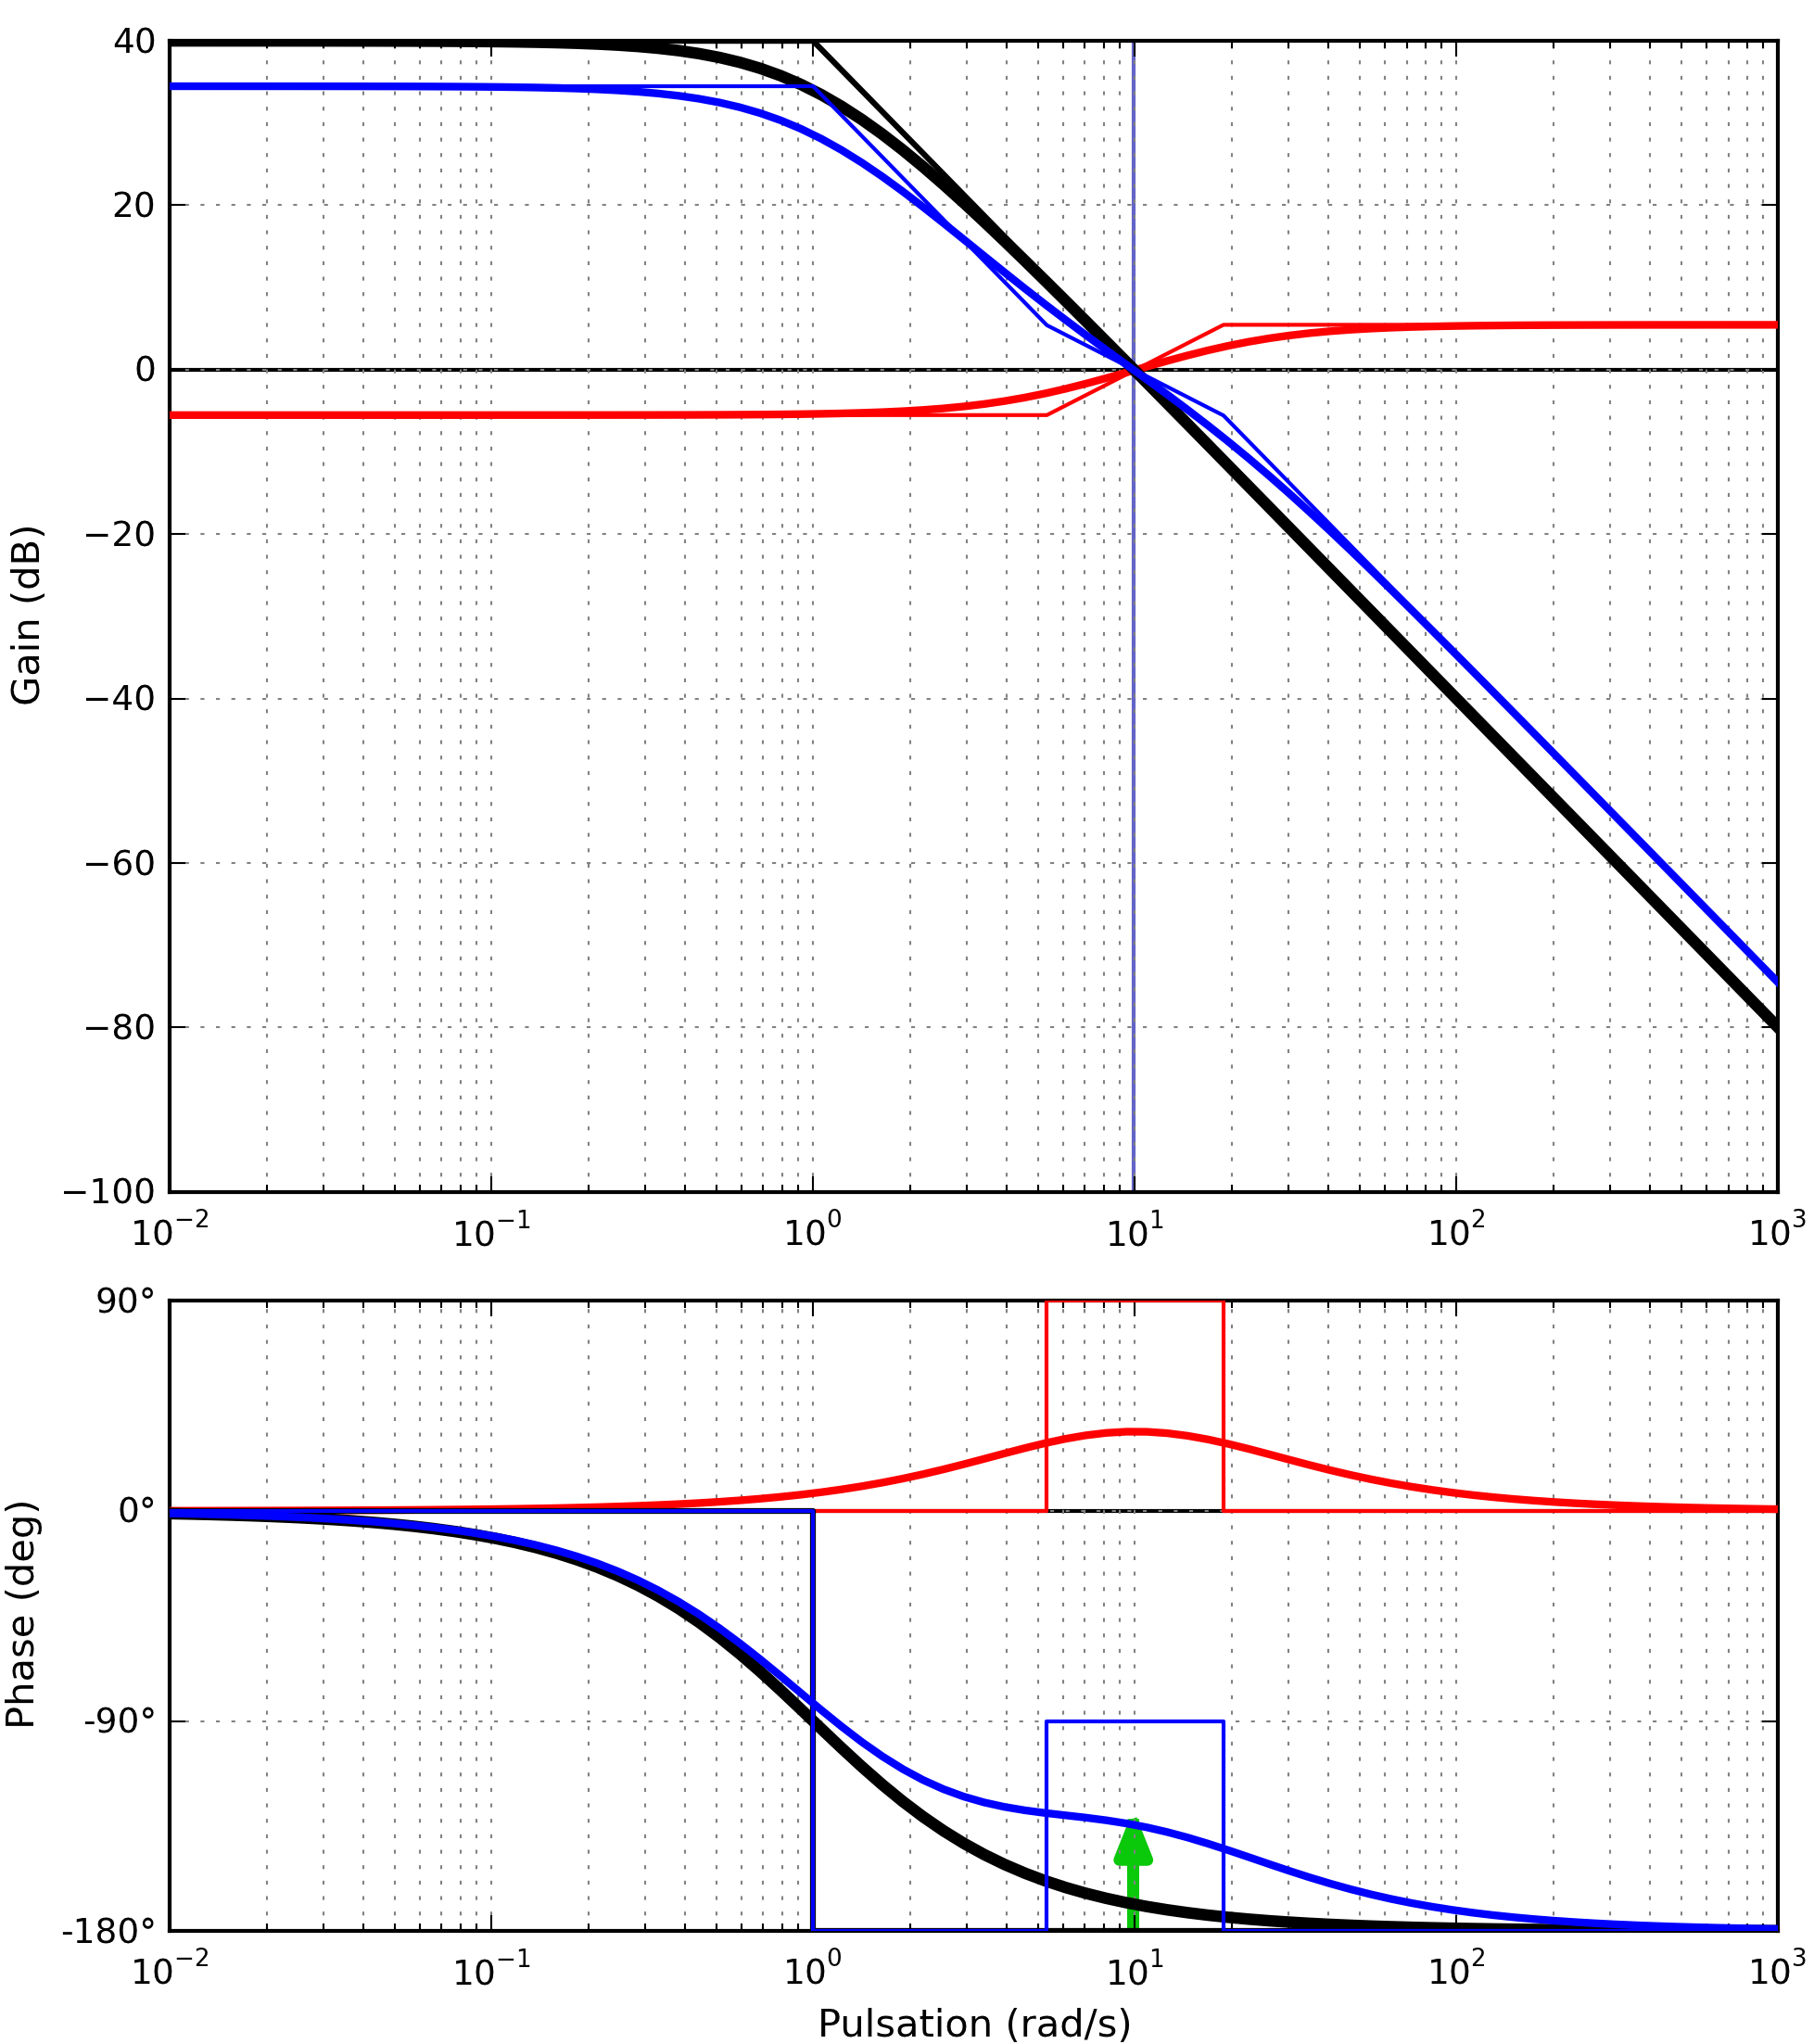
\includegraphics[width=.8\linewidth]{AP_BodeC.png}

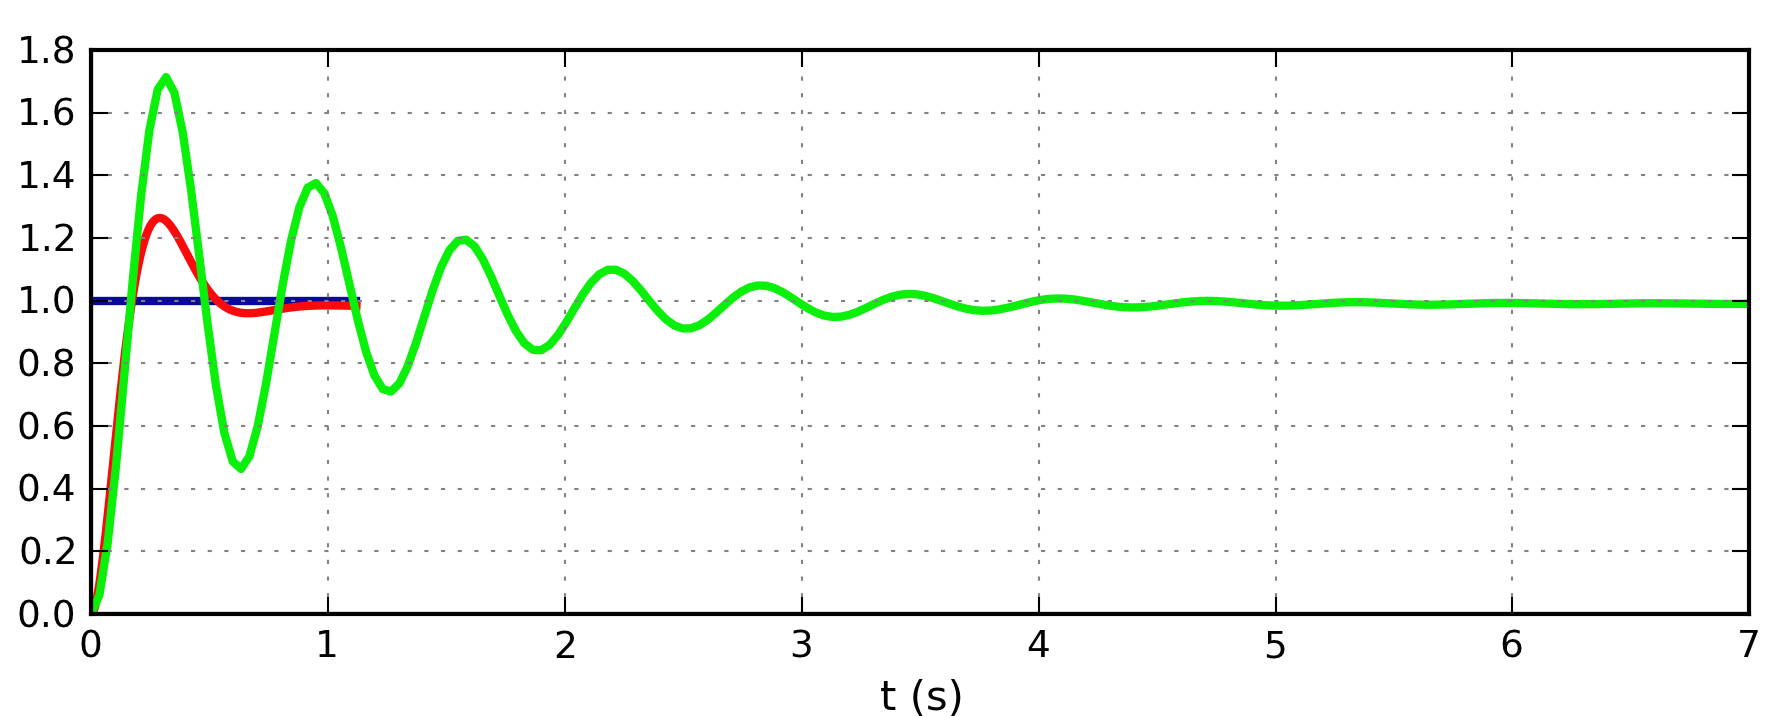
\includegraphics[width=.8\linewidth]{AP_corrige.png}
\end{center}

\fi

\ifprof
\else
%\begin{center}
%\rotatebox{90}{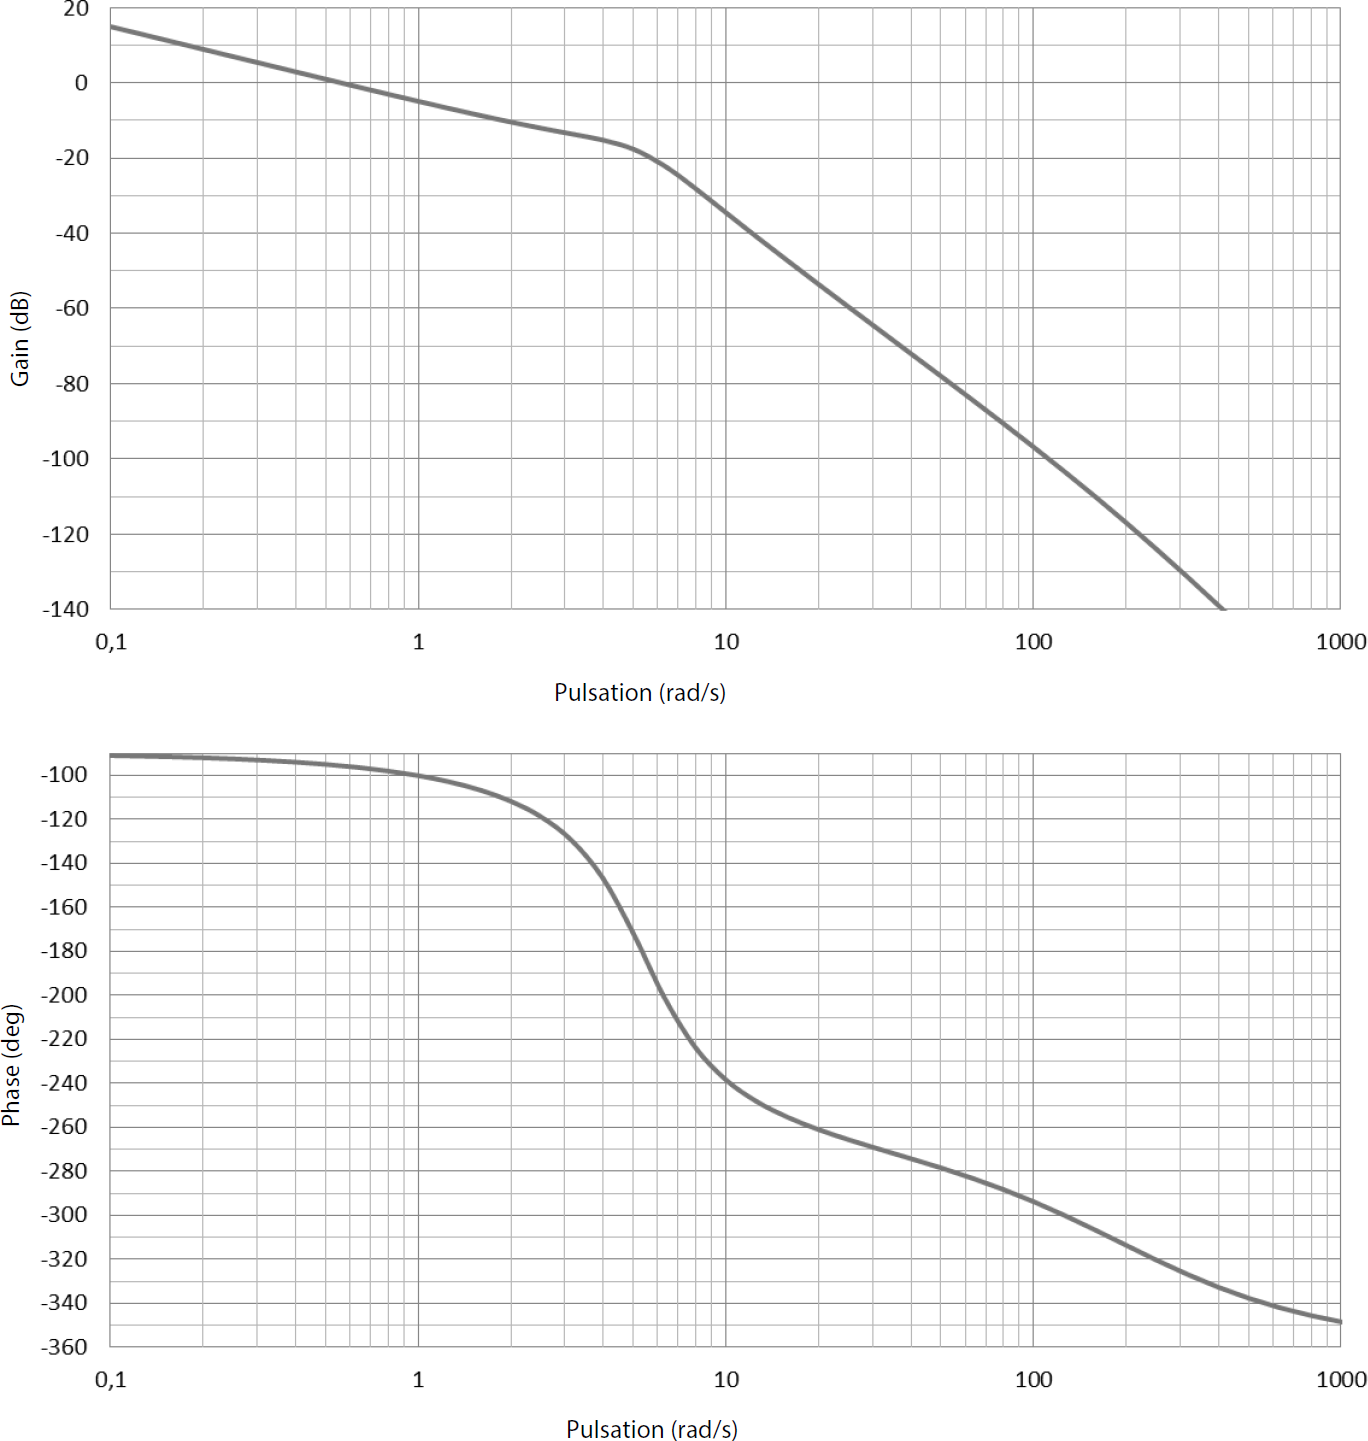
\includegraphics[width=.8\linewidth]{fig_04}}
%
%\rotatebox{90}{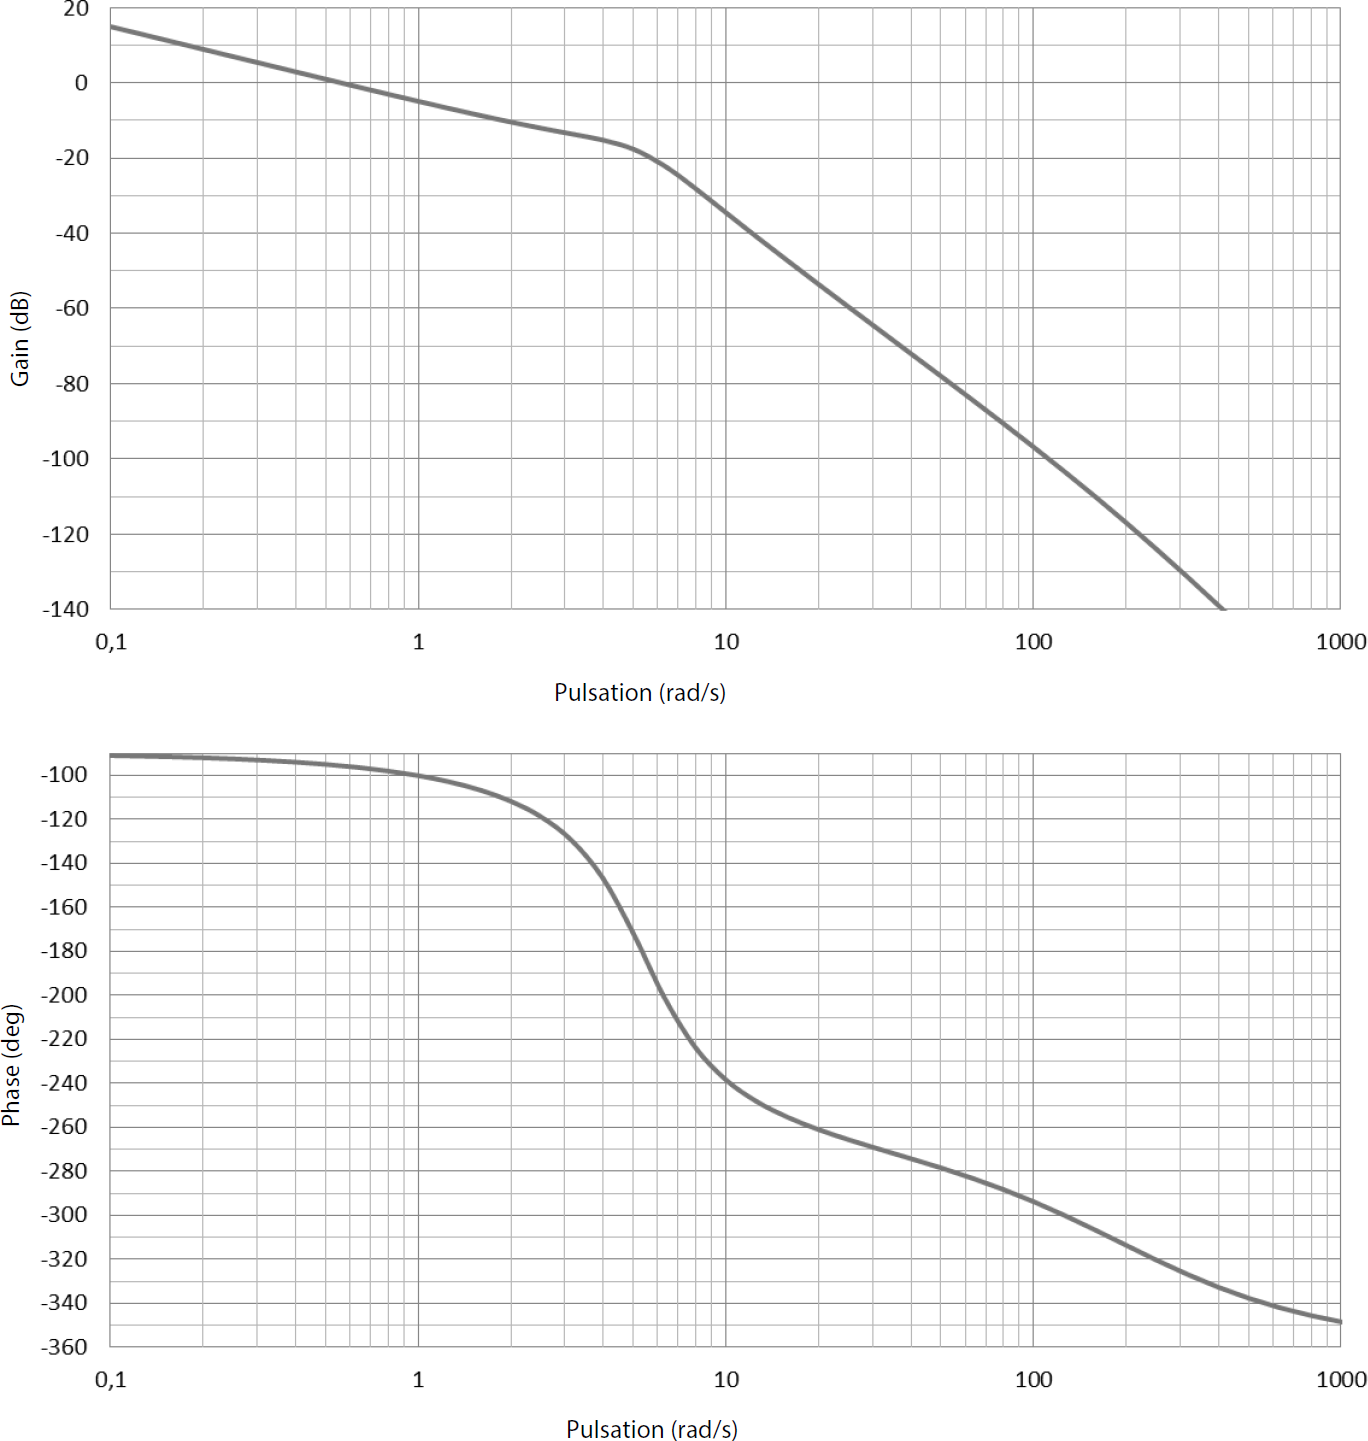
\includegraphics[width=.8\linewidth]{fig_04}}
%\end{center}

\fi


%\end{document}